\chapter{Theoretic Frameworks}
General complexity frameworks for general theoretic areas.


%---------------------------------------------------
%---------------------------------------------------
\section{Meta-complexity}
Some classical problems that are usually reduced to.
%---------------------------------------------------
\subsection{Communication complexity}
\subsubsection{Gap-Hamming-Distance problem}
\begin{prob}[Gap-Hamming\cite{mmmw21}]
\label{ghd}
     Let Alice and Bob be communicating parties who hold vectors $s\in\{\pm1\}^n$ and $t\in\{\pm1\}^n$, respectively. The Gap-Hamming problem asks Alice and Bob to return
     \begin{align*}
         1~if~\langle s,t \rangle\ge \sqrt{n}~~~~~~and~~~~~~-1~if~\langle s,t \rangle\le -\sqrt{n}.
     \end{align*}
     Denote it by $GHD_{n}(x,y)$.
\end{prob}



In general, we need to compute the function $f(x,y)$ for $x\in \mc X, y\in\mc Y$, where $\mc X$ and $\mc Y$ are separate sources and we cannot simultaneously obtain both $x$ and $y$. Instead, we repeatedly communicate information from $x$ to $y$ or from $y$ to $x$, accumulating intermediate information during this process. Finally, we use this accumulative intermediate information to compute $f(x,y)$. The goal is to minimize the number of times of communication or the total amount of communication bits.

To formalize this communication process, a binary tree structure called a "protocol tree" $T$(Fig.\ref{proto_tree}) is used. Each possible value of $f(x,y)$ corresponds to a leaf node $L$ in $T$. The communication complexity is measured by the height $H(T)$ of the tree $T$. Notably, for any node $N$ in $T$, the set $R(N):={(x,y):(x,y)\text{ can reach node $N$}}$ always forms a square, i.e., $R(N)=A\times B$ for some $A\subseteq\mc X$ and $B\subseteq\mc Y$. As a result, the leaf nodes form a rectangular partition of $\mc X\times\mc Y$.

\begin{figure}
  \centering
  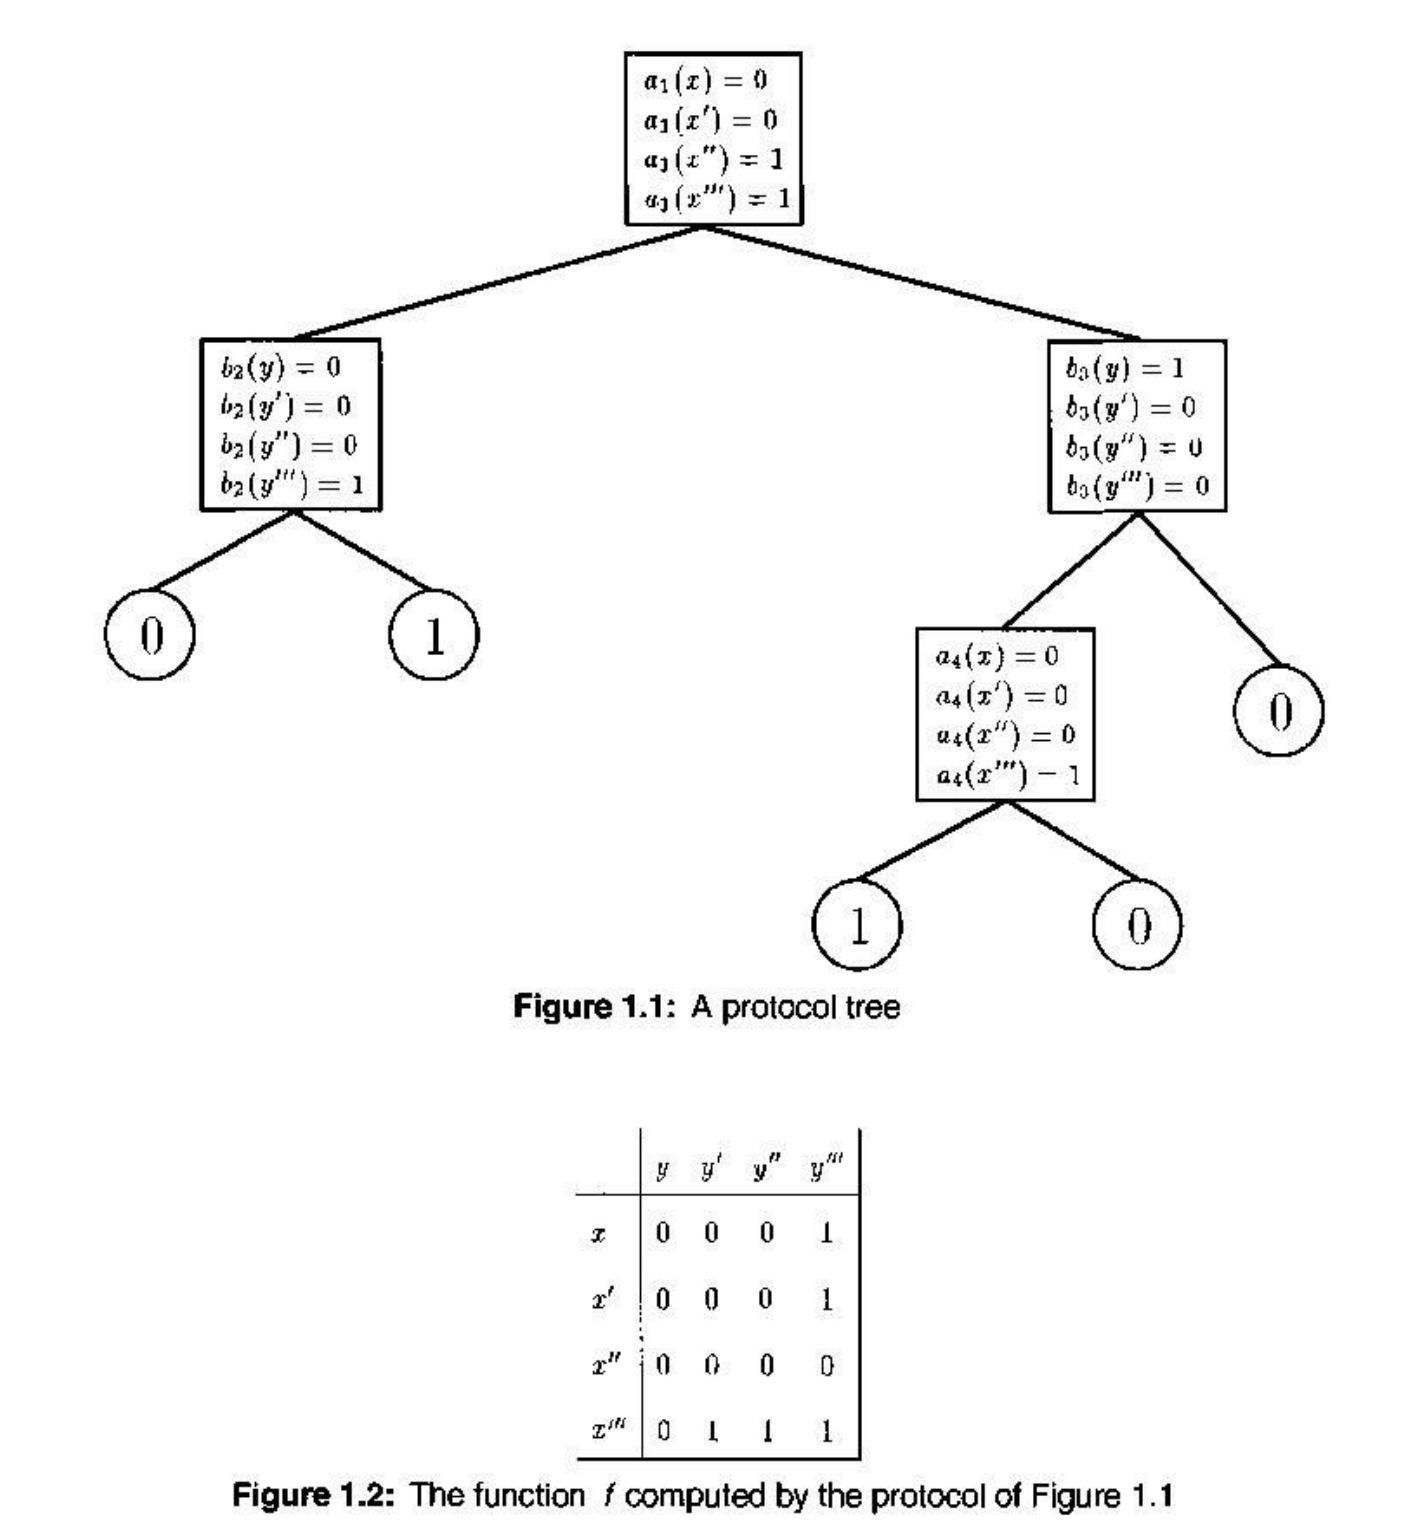
\includegraphics[width=0.5\textwidth]{protocol_tree.png}
  \caption{Protocol tree\cite{kushilevitz1997communication}}
  \label{proto_tree}
\end{figure}

By using the minimum number of square partitions $M_f$ of the function $f(x,y)$, we can derive a lower bound on the communication complexity:

\[
H(T)\ge \log_2 M_f.
\]


\begin{thm}[\cite{cr12}\cite{vidick2012concentration}\cite{sherstov2012communication}]
\label{ghd_lower_bound}
    Any randomized protocol solving problem \ref{ghd} $GHD_n$ with probability $2/3$ needs at least $\Omega(n)$ bits of communication.
\end{thm}

\pfsk{\ref{ghd_lower_bound}}{
The original proof is in \cite{cr12} and \cite{vidick2012concentration} make a simpler one. Here we use proof in \cite{sherstov2012communication}, which is simplist among them.

First, use \textbf{Yao's principle}(theorem \ref{yaoprin}) to reduce the randomness of algorithm to randomness of a distribution $\mu$ of input $(x,y)$. Formally, consider all those deterministic protocol tree $T(x,y)$ such that $\mb P_{(x,y)\sim\mu}[T(x,y)\neq f(x,y)]\le\epsilon$. Denote the minimum complexity(tree height) of such deterministic $T$ by $R_{\mu,\epsilon}(f)$, and denote minimum expectation complexity of random tree with error $\epsilon$ by $C_\epsilon(f)$, we have $C_\epsilon(f)\gtrsim R_{\mu,\epsilon}(f)$. See \cite{yao83} lemma 2 in sect. 3.3 for details.

Then, it suffices to find a hard distribution $\mu$ of $(x,y)$ and lower bound of $R_{\mu,\epsilon}(f)$.
This is done by a trick called \textbf{$\epsilon$-corruption bound}:
\begin{lem}[Yao's corruption bound\cite{sherstov2012communication}]
If $\exists \varepsilon, \delta \in(0,1)$ such that $\mu$ satisfies
$$\mu\left(R \cap f^{-1}(+1)\right)>\varepsilon \mu\left(R \cap f^{-1}(-1)\right)$$
for every rectangle $R \subseteq X \times Y$ with $\mu(R)>\delta$, 
 then $R_{\mu,\xi}(f)\ge\log_2\bbr{\frac{1}{\delta}\left(\mu\left(f^{-1}(-1)\right)-\frac{\xi}{\varepsilon}\right)}$ for small $\xi>0$.
\end{lem}
\noindent Intuitively, the misclassification error in any large rectangle is not so large. Therefore, when total error is a given constant, we can lower bound the number of rectangle partition and thus lower bound the tree height. See \cite{yao83} lemma 3 in sect. 3.3 for originality and details. Usually, people try to directly prove corruption bound for uniformly distribution.

Finally, in our setting, the Gap-Hamming distance problem($GHD_n$) is further reduce to Gap-orthogonality problem($ORT_n$, problem \ref{ort_prob}) with $R_{1/3}(GHD_n)=\Omega(R_{1/3}(ORT_n))$, where $f(x,y)=(-1)\mf 1_{|\langle x,y \rangle|\le\sqrt{n}}+(+1)\mf 1_{|\langle x,y \rangle|\ge2\sqrt{n}}$. 
Note that $f^{-1}(+1)=\{(x,y)||\langle x,y \rangle|\ge2\sqrt{n}\}$, thus the corruption bound intuitively(not so rigorously) means for rectangle $R$ with large probability, we have
\begin{equation}
    \label{anti_concen_ghd}
    \exists c,C>0,~~\mb P_{(x,y)\sim Unif[R]}[|\langle x,y \rangle|>C]\ge c,
\end{equation}
which is essentially a \textbf{anti-concentration analysis}. Choosing uniform distribution is enough, it is proved by \textbf{probabilistic method} with Talagrand's inequalities(corollary \ref{tal_ineq_proj}) and a interesting combinatorial accounting trick:
\begin{lem}[Corruption bound\cite{sherstov2012communication}]
\label{cor_bound}
Let $\mu$ be uniform distribution on $\{\pm1\}^n\times\{\pm1\}^n$ and $R=A\times B$ be a rectangle such that $\mu(R\cap f^{-1}(+1))\le \epsilon\mu(R)$ then $\mu(R)=e^{-\Omega(n)}.$ is small. In other word, if $\mu(R)$ is large, we have corruption bound.
\end{lem}
\pfskm{lemma}{\ref{cor_bound}}{
The anti-concentration inequality is reduced to that, by corollary \ref{tal_ineq_proj} we can find a set $I$ of near-orthogonal vectors of $x\in A$ in rectangle $R=A\times B$ with large probability, and then by some linear algebra and Hoffman-Wielandt inequality, for most of $y\in B$, there must exists a $x'\in I$ such that $|\langle x',y\rangle|$ is large. 
}
\noindent Use the lemma, we compute $C_{1/3}(GHD_n)=\Omega(R_{1/3}(ORT_n))=\Omega(n)$.
}

\begin{rmk}
For general communication problem, the analysis of average-case complexity usually follows the roadmap above:
\begin{enumerate}
    \item Use Yao's principle to reduce the problem with randomized algorithm into a randomized input with deterministic algorithm.
    \item Find the math structures of complexity in setting of deterministic algorithm(In communication problem, it's height of a binary tree whose leaf nodes are rectangle partition).
    \item Abstract these structures into pure math language, and then use fundamental math tool to work it out(In this communication function $f=GHD_n$, the structure is an anti-concentration analysis and tools are some probabilistic methods).
\end{enumerate}
\end{rmk}

\begin{rmk}
Another proof\cite{vidick2012concentration} use a different description of the anti-concentration(theorem \ref{large_overlap}) in corruption bound \eqref{anti_concen_ghd}, where they consider general vectors $x,y\in\R^n$($\mc X,\mc Y, R$ may be continuous).
\end{rmk}
%---------------------------------------------------
\subsubsection{Approximate-Orthogonality problem}
\begin{prob}[\cite{chakrabarti2012information}\cite{woodruff2022optimal}]
\label{ort_prob}
Let Alice and Bob be communicating parties who hold vectors $s\in\{\pm1\}^n$ and $t\in\{\pm1\}^n$, respectively. The Approximate-Orthogonality problem asks Alice and Bob to return
\begin{align*}
    1~if~|\langle s,t \rangle|\le b\sqrt{n}~~~~~~and~~~~~~-1~~~otherwise.
\end{align*}
Denote it by $ORT_{b,n}(x,y)$.
\end{prob}

\begin{thm}[\cite{chakrabarti2012information}\cite{woodruff2022optimal}]
\label{ort_complexity}
Any randomized protocol solving problem \ref{ort_prob} $ORT_{b,n}$ with probability at least $\Phi(2.01\max\{66,b\})$($b>1/5$) needs at least $\Omega(n)$ bits of communication. Where $\Phi(x)$
is $c.d.f.$ of $\mc N(0,1)$.
\end{thm}
\pfsk{\ref{ort_complexity}}{
    \xb{based on anti-concentration lemma \ref{ort_anti_concen}}
}
%---------------------------------------------------
\subsubsection{Gap-Equality problem}
\begin{prob}[\cite{woodruff2022optimal}]
\label{eq_prob}
Let Alice and Bob be communicating parties who hold vectors $s\in\{0,1\}^n$ and $t\in\{0,1\}^n$ with either $s=t$ or $\|s-t\|_2^2=n/2$, respectively. The Gap-Equality problem asks Alice and Bob to return
\begin{align*}
    1~if~s=t~~~~~~and~~~~~~-1~~~otherwise.
\end{align*}
Denote it by $EQ_{n}(x,y)$.
\end{prob}
\begin{thm}
\label{eq_complexity}
Any deterministic protocol solving problem \ref{eq_prob} $EQ_n$ needs at least $\Omega(n)$ bits of communication.
\end{thm}

%---------------------------------------------------
\subsubsection{Augmented Indexing problem}
\begin{prob}[\cite{woodruff2022optimal}]
\label{ind_prob}
Given set $\mc U$ and an elements $\perp\notin\mc U$.
Let Alice and Bob be communicating parties who hold vectors $s\in\mc U^n$ and $t\in\{\mc U\cup\{\perp\}\}^n$
with either $s_k=t_k,~k<i$, $t_i\in\mc U$ and $y_{i+1}=\cdots=y_n=\perp$ for some unique $i$.
The Gap-Equality problem asks Alice and Bob to return
\begin{align*}
    1~if~s_i=t_i~~~~~~and~~~~~~-1~~~otherwise.
\end{align*}
Denote it by $IND_{n,\mc U}(x,y)$.
\end{prob}
\begin{thm}
\label{ind_complexity}
Any one-way(only one people can send message to the other people) randomized protocol solving problem \ref{ind_prob} $IND_{n,\mc U}(x,y)$ with error $\delta\le\frac{1}{4|\mc U|}$ needs at least $n\log|\mc U|/2$ bits of communication.
\end{thm}

%---------------------------------------------------
\subsection{Spiked wishart matrix testing}
\begin{prob}[Spiked wishart matrix\cite{mmmw21}\cite{pwbm18}]
\label{spiked_wishart}
Let $n=1/\epsilon$ and let $z\in\R^n$ be a uniformly random unit vector. Let $N\in\R^{n\times m}$ be $m$ $i.i.d$ Gaussian vector drawn from an $n$-dimensional $\mc N(0,C)$, where $C=I$ or $I-zz^T$. Use $N$ to identify $C$.
\end{prob}

\begin{thm}[\cite{mmmw21}]
\label{spiked_whishart_lower_bound}
To solve problem \ref{spiked_wishart} with probability at least $2/3$, we need at least $m=\Omega\bbr{\frac{1}{\epsilon}}$.
\end{thm}
\pfsk{\ref{spiked_whishart_lower_bound}}{First, let $P$ denote the distribution of $N$ under null hypothesis $C=I$, and $Q$ denote the distribution of $N$ under alternative hypothesis $C=I-zz^T$. Any testing statistics $\phi$ outputs $1$ for $Q$ and $0$ for $P$. It suffices to bound the total variation distance $d_{TV}(P,Q)$, since its control the summation of Type-1 and Type-2 errors
\begin{align*}
    \min_\phi\bbwr{P(\phi=1)+Q(\phi=0)}=1-d_{TV}(P,Q).
\end{align*}

Then, by Pinsker's inequality, we have $d_{TV}(Q,P)\le\sqrt{\frac{1}{2}D_{KL}(Q||P)}\le\sqrt{\frac{1}{2}D_{\chi^2}(Q||P)}.$
Therefore it suffices to upper bound $D_{\chi^2}(Q||P)=\int_{N}\bbr{\frac{Q(N)}{P(N)}}^2P(N)dN - 1$. By theorem \ref{spiked_gaussian_chi_dist} with $\beta=-1$ and spiked prior $z$, we have
\begin{align*}
    D_{\chi^2}(Q||P) = \mb E_{v,v'}\bbfr{(1-\langle v,v' \rangle^2)^{-m/2}}-1,
\end{align*}
where $v,v\stackrel{\mathrm{dist}}{=}z$ are uniformly random unit vectors. Therefore, by classical results of random unit vectors, $p.d.f.$ of $x:=\langle v, v'\rangle$ is $p(x)=\frac{\Gamma(n-1)}{2\Gamma((n-1)/2)^2}\bbr{\frac{1-x^2}{4}}^{(n-1)/2-1}$.

Finally, direct calculation yields, if $m=O\bbr{1/\epsilon}$, $\mb E_{v,v'}\bbfr{(1-\langle v,v' \rangle^2)^{-m/2}}<6/5$ and thus $d_{TV}(Q,P)<1/3$. Therefore, one of Type-1 and Type-2 errors must be larger than $1/3$.
}

\begin{prob}[\cite{jpwz21}]
    \label{hard_psd_testing}
    Given $\delta\in(0,1/2)$, set $n=\log(1/\delta)$. Independently take $g\sim\mc N(0,I_n)$ and $G\in\R^{n\times n}$ with $i.i.d.$ $\mc N(0,1)$ entries. Let $W=G+G^T$. Consider two distributions:
    \begin{itemize}
        \item Distribution $P$: $C\log^{3/2}(1/\delta)\cdot\frac{1}{\|g\|_2^2}gg^T + W + 6\sqrt{\log(1/\delta)}I_n$ for some fixed constant $C>0$.
        \item Distribution $Q$: $W + 6\sqrt{\log(1/\delta)}I_n$.
    \end{itemize}
    Use \textbf{non-adaptive} queries $q_1,...q_m$ and oracles $Aq_1,...,Aq_m$ to distinguish $P$ and $Q$. In other word, take a matrix $Q\in\R^{n\times m}$ as query and $AQ$ as oracle.
\end{prob}
\begin{thm}[\cite{jpwz21}]
    \label{hard_psd_testing_bound}
    Any randomized algorithm solving problem \ref{hard_psd_testing} with probability $1-\delta$ need at least $m=\Omega\bbr{\frac{\log(1/\delta)}{\log\log(1/\delta)}}$ queries. 
\end{thm}
\pfsk{\ref{hard_psd_testing_bound}}{
Similar to the proof of theorem \ref{spiked_whishart_lower_bound}, it is naturally to consider bounding the total variation $d_{TV}(P,Q)$, and by rotational invariance we WLOG assume $Q=E_m$, the first $m$ standard basis vectors. 

First, denote by $P',Q'$ the distribution of $BQ$($B\sim P$ or $Q$ respectively). Let $L_{P'},L_{Q'}\in\R^{l}$ be vectorization of matrices from $P',Q'$(remove the redundant variable, since $B$ is symmetric), where $l=n+(n-1)+\cdots (n-m+1)$. Observe that conditioned on a realization $g$ we have
\begin{align*}
    d_{KL}(P',Q'|g)&\le d_{KL}(L_{P'},L_{Q'}|g)
    \le \|\mb EL_{P'} - \mb EL_{Q'}\|_2^2=\sum_{i=1}^m\left\|C\log^{3/2}(1/\delta)\frac{gg^T}{\|g\|_2^2}e_i\right\|_2^2=C^2\log^{3}(1/\delta)\frac{\|g^T Q\|_2^2}{\|g\|_2^2}.
\end{align*}
The first inequality use data processing inequality(theorem \ref{data_process}) and the second inequality uses theorem \ref{gauss_kl}.

Then, find a typical event $\mc E$ with positive probability. We take $\mc E=\bbwr{\frac{\|g^T Q\|_2^2}{\|g\|_2^2}\le\frac{1}{50C^2n^3}}$ and show that $\mb P(\mc E)\ge 10\delta$ if we only take $m=O\bbr{\frac{\log(1/\delta)}{\log\log(1/\delta)}}$ queries. Indeed, assume $m\le n/2$
$$
\mb P(\mc E)\ge \mb P(\|g\|_2^2\ge n/2|\|g^T Q\|_2^2\ge 1/(100C^2n^2))\cdot\mb P(\|g^T Q\|_2^2\ge 1/(100C^2n^2))
= \Omega(1)\cdot\Omega((\frac{1}{n\sqrt{m}})^m)=\Omega(e^{-\frac{m}{2}\log(n^2m)}).
$$
Therefore, when $m=O\bbr{\frac{\log(1/\delta)}{\log\log(1/\delta)}}$, $\mb P(\mc E)\ge 10\delta$.

Finally, conditioned realization $g\in\mc E$, we have the total variation $d_{TV}(P',Q'|g)\le\sqrt{d_{TV}(P',Q'|g)/2}\le 1/3$ by Pinsker's inequality. This means $\mb P[\text{the algorithms make mistake}|g]\ge 1/3$ under $P'$ or $Q'$. Since $\mb P(\mc E)\ge 10\delta$, we have $\mb P[\text{the algorithms make mistake}]\ge \delta$ under $P$ or $Q$ if we only take $m=O\bbr{\frac{\log(1/\delta)}{\log\log(1/\delta)}}$ queries.
}
\begin{rmk}
This bound is independent of error $\epsilon$. Informally, this is because there is a sharp phase transition due to its mathematical structure. Similar structures can be found in proof of theorem \ref{tr_est_ada_schatten_p}, provided by Gap-Equality problem \ref{eq_prob}'s sharp contrast.
\end{rmk}
\xb{consider directly bound $d_{TV}(P,Q)\le 1-2\delta$ instead?}


%---------------------------------------------------
%---------------------------------------------------
%---------------------------------------------------
\section{Informational-computational gap}
The informational-computational gap refers to the phenomenon where certain statistical problems are informationally solvable, yet lack efficient (polynomial-time) algorithms in some regimes.

Three major research direction: \xb{need to add citations below, see intro of \cite{bandeira2022franzparisi} and appendix A of COLT verision of \cite{brennan2020reducibility}}
\begin{enumerate}
    \item Reduction form different average-case problems. reduced them to some classical forms, e.g. planted cliques.
    \item Prove the failure of the problems under some general classes of algorithms, e.g. sum of squares, low degree polynomial, statistical query model etc.
    \item Analyze the phenomena appeared in hard regime, e.g. overlap gap property, low degree likelihood ratio etc.
\end{enumerate}
%---------------------------------------------------
%---------------------------------------------------
\subsection{Average-case reduction}
Three principles\cite{brennan2020reducibility}
\begin{enumerate}
    \item Correctly map the distribution of noise and signal
    \item Lower bound from reduction must be tight(achieved by best known efficien algorithm)
    \item Tackle the different amount of parameters of the problem to reduce, e.g. biclustering problem has 2 parameters while planted clique has only one.
\end{enumerate}
%---------------------------------------------------
\subsubsection{An example of reduction: reduce biclustering to planted cliques}
This section is mainly from \cite{avg_redu_1} and \cite{avg_redu_2}.

%---------------------------------------------------
\subsubsection{Problems}

\begin{prob}[Biclustering]
\label{bc_prob}
Given a random matrix $X\in\rn n $, a biclustering problem with parameter $n,k,\lambda$ is the following hypothesis testing problem
\begin{itemize}
    \item $H_0$: $X_{ij}\stackrel{i.i.d.}{\sim}\mc N(0,1)$
    \item $H_1$: there exists $S,T\stackrel{i.i.d.}{\sim}\binom{[n]}{k}$, $X_{ij}\stackrel{i.i.d.}{\sim}
    \begin{cases}
        \mc N(\lambda,1) & \text{if $i\in S,j\in T$,}\\
      \mc N(0,1) & \text{otherwise.}
    \end{cases}$ 
\end{itemize}
Denote it by $BC(n,k,\lambda)$.
\end{prob}

\begin{prob}[Planted cliques]
\label{pc_prob}
Given a random graph $G=(V,E)$, a planted cliques problem with parameter $n,k$ is the following hypothesis testing problem
\begin{itemize}
    \item $H_0$: $E_{ij}\stackrel{i.i.d.}{\sim}Ber(1/2)$ for $i>j$,
    \item $H_1$: there exists $U\sim\binom{[n]}{k}$, $E_{ij}=
    \begin{cases}
      1 & \text{if $i,j\in U$,}\\
      Ber(1/2) & \text{otherwise.}
    \end{cases}$ 
\end{itemize}
Denote it by $PC(n,k)$.
\end{prob}

\begin{figure}
    \centering
    \begin{subfigure}[b]{0.3\textwidth}
        \centering
        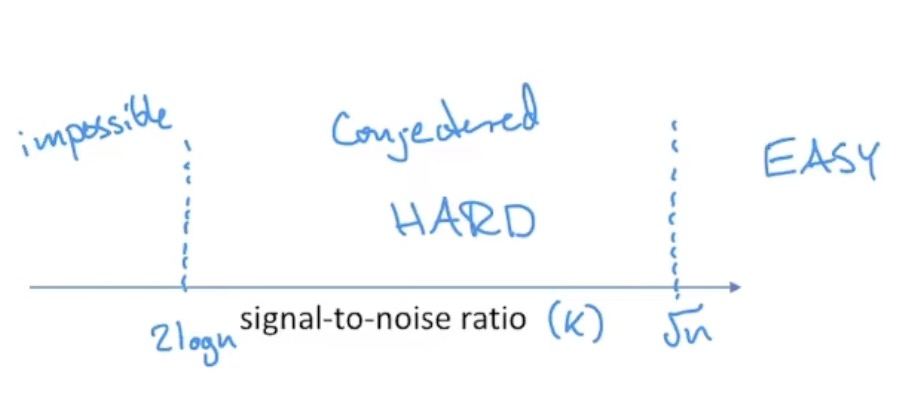
\includegraphics[width=\textwidth]{pc.jpg}
        \caption{$PC(n,k)$, picture from \cite{info_comp_alg_equiv}}
        \label{pc_threshold}
    \end{subfigure}
    \hspace{3cm}
    \begin{subfigure}[b]{0.3\textwidth}
        \centering
        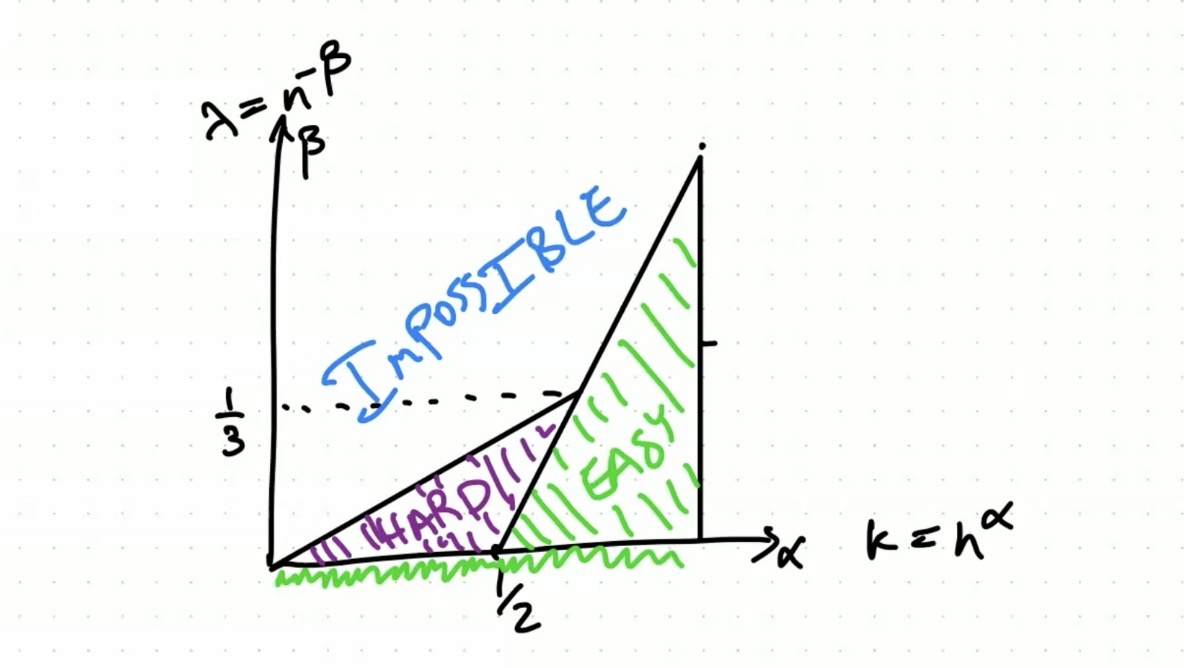
\includegraphics[width=\textwidth]{bc.jpg}
        \caption{$BC(n,k,\lambda)$, picture from \cite{avg_redu_1}}
        \label{bc_threshold}
    \end{subfigure}
    \caption{Phase transition of informational and computational thresholds}
    \label{pc_bc_threshold}
\end{figure}
The phase transition of informational thresholds of both problems can be proved. However, we currently only have evidence for computational thresholds, lacking definitive proof.
\begin{itemize}
    \item For $PC(n,k)$ with $k=n^{\alpha}$($\alpha>1/2$), the statistics $T(G)=\mf{1}_{\text{max degree}\ge n/2+\sqrt{Cn\log n}}$ for sufficiently large constant $C$ succeeds to detect the hypothesis with polynomial time.
    This is because
    \begin{itemize}
        \item Under $H_0$, $\mb P(T=1)\le n\mb P(Ber(n,1/2)\ge n/2+\sqrt{Cn\log n})\le n\cdot n^{-2}\rightarrow 0$;
        \item Under $H_1$, 
        \begin{align*}
            \mb P(T=0)&\le \mb P(\text{for }i\text{ in the planted clique }deg(i)\le n/2+\sqrt{Cn\log n})\\
            &=\mb P(Ber(n-k,1/2)\le n/2-k+\sqrt{Cn\log n})^k\le \mb P\left(|\sum_{i=1}^{n-k}X_i-\mb EX_i|\ge k/2+\sqrt{Cn\log n}\right)^k\\
            &\le 2^ke^{-c\frac{k^2}{n}\cdot k} \rightarrow 0.
        \end{align*}
    \end{itemize}
    
    But there is no efficient algorithm for $\alpha\le 1/2$.

    \item For $BC(n,k,\lambda)$\cite{ma2015computational} with $k=n^\alpha$ and $\lambda=n^{-\beta}$,we first show some poly-time statistics in easy regime
    \begin{itemize}
        \item if $\beta< 0$, the maximum statistics $T_{max}(X)=\max_{i,j}X_{i,j}=\begin{cases}
            O(\sqrt{\log n}) & \text{under } H_0 \\
            \Omega(\lambda) & \text{under } H_1.
        \end{cases}$ 
        Thus it succeeds to detect the hypothesis with polynomial time.
        \item if $\beta> 0$, the average statistics $T_{avg}(X)=\frac{1}{n}\sum_{i,j}X_{i,j}=\begin{cases}
            \mc N(0,1) & \text{under } H_0 \\
            \mc N(\frac{k^2\lambda}{n},1) & \text{under } H_1.
        \end{cases}$
        Thus it succeeds to detect the hypothesis with polynomial time when $\beta<2\alpha - 1$.
    \end{itemize}
    But there is no efficient algorithm in regime among impossible regime and easy regime, which is conjectured to be hard.
    Though there does have some statistics solve the problem in this regime, they are not poly-time. 
    
    For example, the searching statistics $T_{search}=\frac{1}{k}\max_{|S|=|T|=k}\sum_{i\in S,j\in T}X_{ij}\begin{cases}
        =O(\sqrt{k\log n}) & \text{under } H_0 \\
        \ge \frac{k\lambda}{\sqrt{\log n}} ~w.h.p.~& \text{under } H_1
    \end{cases}$, where the first case is because $T_{search}\approx\max\text{ of }\binom{n}{k}^2~\mc N(0,1)$ 
    and the second case is because $T\ge \frac{1}{k}\sum_{i,j:X_{i,j}\sim\mc N(\lambda,1)}X_{i,j}\sim \mc N(k\lambda,1)$. 
    
    Therefore $\lambda\gg\frac{\log n}{\sqrt{k}}$ or $\beta<\alpha/2$ can solve the problem. Later we will see this is actually informational boundary.
\end{itemize}

\begin{thm}
    \label{pc_info_threshold}
    For $PC(n,k)$, the informational boundary is $2\log n$.
\end{thm}
\pfsk{\ref{pc_info_threshold}}{
    The proof is based on second moment method, see \cite{planted_clique_proof} for details.
}


\begin{thm}
    \label{bc_info_threshold}
    For $BC(n,k,\lambda)$, the informational boundary are the line segments shown in figure \ref{bc_threshold}.
\end{thm}
\pfsk{\ref{bc_info_threshold}}{
    The proof is to prove $d_{TV}(H_0,H_1)\rightarrow 0$, see \cite{brennan2019reducibility} theorem 40 for details.
}

\begin{conj}
    The phase transition of computational thresholds are in figure \ref{pc_bc_threshold}.
\end{conj}

\vspace{10pt}

%---------------------------------------------------
\subsubsection{Reduction}

We will show how to derive computational boundary between easy and hard regime of $BC(n,k,\lambda)$, assuming hardness result of $PC(n,k)$. But first we need the following prelinminary knowledge.
\begin{defn}[Worst-case reduction]
Let $P, P'$ be two worst-case problems. We say that $P$ reduces to $P'$, denoted by $P \leq_p P'$ if there is a polynomial-time computable algorithm $\mc A$ such that
$$
\mc A(P) = P',
$$
which means operating on the problem instance of $P$ to construct a problem instance of $P'$.
We say that $P$ and $P'$ have equivalent complexity if $P \leq_p P'$ and $P' \leq_p P$.
\end{defn}
\textbf{Example.} Reduce 3-SAT to independnent set problem, where the constructed graph $G$ has an independent set of size $k$ iff SAT formula $\Phi$ has a satisfying assignment. 

\textbf{Remark.} Intuitively, we may think hardness as \textbf{"amount of algorithms to solve the problem"}. In that way, $\mc A(P) = P'$ means all algorithms that can solve $P'$, can also solve $P$ combining with $\mc A$. Therefore, algorithms for $P$ is no fewer than $P'$ and $P$ is no harder than $P'$.

Compared to worst-case reduction, average-case reduction is significantly more complex because it involves not only mapping between structurally similar objects, but also mapping between distributions such that their statistical distances are small.

\begin{lem}[Total variation]
    Given two distribution $\mu$ and $\nu$, the total variation distance $d_{TV}(\mu,\nu)$ has the following equivalent definitions
    \begin{align*}
        d_{TV}(\mu,\nu) &= \frac{1}{2}\|\mu-\nu\|_1 
                        = \frac{1}{2}\int |f(x)-g(x)|dx ~~\text{if they have density $f,g$}\\
                        &= \sup_{E}|\mu(E) - \nu(E)| 
                        = \inf_{(X,Y),X\sim\mu,Y\sim\nu}\mb{P}(X\neq Y)\\
                        &=1- \min_{\phi:\phi\text{ is a testing statistics}}\{\mu(\phi\text{ indicates }\nu)+\nu(\phi\text{ indicates }\mu)\}.
    \end{align*}
\end{lem}

\begin{defn}[Reduction]
    Let $P, P'$ be two average-case problems. The reduction with error $\epsilon$ from $P$ to $P'$ is an polynomial-time computable algorithm $\mc A$ such that
    \[
        d_{TV}(\mc A(P), P')\le\epsilon.
    \]
\end{defn}

\begin{lem}[Properties of reduction]
    \label{property_redu}
    \begin{itemize}
        \item  Let algorithm $\mc A$ be reduction with error $\epsilon$ from $P$ to $P'$. If algorithm $\Phi$ solves $P'$ with probability $\delta$, then $\Phi\circ\mc A$ solves $P$ with probability $\delta+\epsilon$.
        \item  Let algorithm $\mc A_1$ be reduction with error $\epsilon_1$ from $P$ to $P_1$, and algorithm $\mc A_2$ be reduction with error $\epsilon_2$ from $P_1$ to $P_2$. Then $\mc A:=\mc A_2\circ \mc A_1$ is reduction with error $\epsilon_1+\epsilon_2$ from $P$ to $P_2$.
    \end{itemize}
\end{lem}
\pfm{lemma}{\ref{property_redu}}{
    \begin{enumerate}
        \item $\mb P_{X\sim P}(\phi\circ A \text{ solves } X)\le d_{TV} + \mb P_{Y\sim P'}(\phi \text{ solves } Y)\le \epsilon + \delta$.
        \item $d_{TV}(\mc A_2\circ\mc A_1(P),P_2)\le d_{TV}(\mc A_2\circ\mc A_1(P),\mc A_2(P_1)) + d_{TV}(\mc A_2(P_1),P_2)\le \epsilon_1+\epsilon_2$ by data processing inequality.
    \end{enumerate}
}

Now, we try to reduce problem $P=PC(n,k)$ to problem $P'=BC(n,k,\lambda)$. 
It's natural to map adjacency matrix of the random graph in $P$ to random matrix in $P'$. 
However, it's not trivial since the randomness are not the same, and the adjacency matrix is symmetric and without diagonal entries.

To solve these problems, the reduction is constructed by the following steps:
\begin{enumerate}
    \item Map Bernoulli variables to Gaussian variables.
    
        To find a mapping $\Phi$ such that $\Phi(1)=\mc N(\lambda,1)$ and $\Phi(Ber(1/2))=\mc N(0,1)$. 
        Denote p.d.f of $\mc N(\lambda,1),\mc N(0,1)$ by $P,Q$ respectively. Then p.d.f. of $\Phi(0)$ should be $2Q-P$.

        However, this density may not be positive all the time. Therefore we take truncation p.d.f.\ such that $\Phi(0)\sim\rho(x):=\frac{1}{Z}(2Q(x)-P(x))\mf{1}_{2Q-P>0}$ instead.
        Though it's not exact mapping we want, but fortunately we have $\Phi(Ber(1/2))\approx Q$.
        \begin{lem}
            \label{ber_to_gau_trunc_approx}
            If $\lambda\le O(\frac{1}{\sqrt{\log n}})$, then $d_{TV}(\Phi(Ber(1/2)),Q)=o(n^{-3})$.
        \end{lem}
        \pfskm{lemma}{\ref{ber_to_gau_trunc_approx}}{
            First note that the support is $(-\infty,\frac{\lambda}{2}+\frac{1}{\lambda}\log 2)$, then direct calculation yields $Z=1+o(n^{-3})$.
            Therefore $d_{TV}=\frac{1}{2}\left(\int|\frac{v(x)+P(x)}{2}-Q(x)|\mf 1_{2Q-P> 0}dx + \int|\frac{P(x)}{2}-Q(x)|\mf 1_{2Q-P< 0}dx \right)= o(n^{-3})$.
        }
        \begin{lem}
            \label{tv_tensor}
            If $X_1\indep X_2$ and $Y_1\indep Y_2$, then $d_{TV}((X_1,X_2),(Y_1,Y_2))\le d_{TV}(X_1,Y_1)+d_{TV}(X_2,Y_2)$.
        \end{lem}
        Now we construct matrix $W\in\rn n$, such that $W_{ij}=W_{ji}=\Phi(E_{ij})$ for $i\neq j$ otherwise $0$.
        By tensorization lemma \ref{tv_tensor}, the total variation distance between upper triangle of $W$ and $X$ is
        \[d_{TV}(W_{upper},X_{upper})\le o(n^2\cdot n^{-3})=o(n^{-1}).\]

    \item Clone Gaussian variables to symmetrize.
        
        There is an algorithm to clone independent copies of any gaussian variable.
        \begin{thm}
            \label{gauss_clone} 
            Let $X\sim\mc N(\mu,\sigma^2)$ as input, we can output $\mc N(\frac{\mu}{\sqrt{2}},\sigma^2)^{\otimes 2}$.
        \end{thm}
        \pfsk{\ref{gauss_clone}}{
            Let $Z\indep X$ with $Z\sim\mc N(0,\sigma^2)$, 
            then the joint distribution of $\frac{1}{\sqrt{2}}\begin{bmatrix}
                1 & 1\\
                1 & -1
            \end{bmatrix}\begin{pmatrix}
                X \\
                Z
            \end{pmatrix}$ is what we want.
        }
        Now we take an antisymmetric matrix $A$ with i.i.d. $\mc N(0, 1)$ random variables below
        its main diagonal and set $W\leftarrow \frac{1}{\sqrt{2}}(W+Z)$. Then we have the total variation distance between off-diagonal entries of $W$ and $X$ is 
        $$d_{TV}(W_{off},X_{off})=o(n^{-1})$$.

    \item Add diagonal randomness.
        
        Fill the diagonal entries of $W$ with $i.i.d.$ $\mc N(0,1)$ and permutation the columns randomly. The following techical lemma guarantee the total variation may not be too large.
        \begin{lem}[lemma 8 in \cite{brennan2019reducibility}]
            \label{off_diag_permut}
            Given distribution $P$ and $Q$. Let $M$ be random matrix whose diagnoal entries are $i.i.d$ samples from $P$ and off-diagonal entries are $i.i.d$ samples from $Q$.
            Choose a permutation $\sigma$ on $[n]$ uniformly at random, permutate columns of $M$ to yield $M_{\sigma}$. Then, we have
            \[
              d_{TV}(M_\sigma,Q^{\otimes n\times n})\le \sqrt{\frac{\chi^2(P,Q)}{2}}.  
            \]
        \end{lem}
        \pfskm{lemma}{\ref{off_diag_permut}}{
            First, note that $d_{\mathrm{TV}}\left(M_\sigma, Q^{\otimes n \times n}\right) \leq \frac{1}{2} \sqrt{\chi^2\left(M_\sigma, Q^{\otimes n \times n}\right)}$. 
            
            Then direct calculation yields
            \begin{align*}
                &\chi^2\left(M_\sigma, Q^{\otimes n \times n}\right)+1
                =\int \frac{\mathbb{E}_\sigma\left[\mathbb{P}_{M_\sigma}(X \mid \sigma)\right]^2}{\mathbb{P}_{Q^{\otimes n \times n}}(X)} d X
                =\mathbb{E}_{\sigma, \sigma^{\prime}} \int \frac{\mathbb{P}_{M_\sigma}(X \mid \sigma) \mathbb{P}_{M_{\sigma'}}\left(X \mid \sigma^{\prime}\right)}{\mathbb{P}_{Q^{\otimes n \times n}}(X)} d X\\
                &= \mathbb{E}_{\sigma, \sigma^{\prime}} \int\left(\prod_{i: \sigma(i)=\sigma^{\prime}(i)} 
                \frac{P\left(X_{i \sigma(i)}\right)^2}{Q\left(X_{i \sigma(i)}\right)}\right)\left(\prod_{i: \sigma(i) \neq \sigma^{\prime}(i)} P\left(X_{i \sigma(i)}\right)\right) 
                 \times\left(\prod_{i: \sigma(i) \neq \sigma^{\prime}(i)} P\left(X_{i \sigma^{\prime}(i)}\right)\right)\left(\prod_{j \neq \sigma(i), j \neq \sigma^{\prime}(i)} Q\left(X_{i j}\right)\right) d X \\
                & =\mathbb{E}_{\sigma, \sigma^{\prime}}\prod_{i: \sigma(i)=\sigma^{\prime}(i)}\left(\int \frac{P\left(X_{i \sigma(i)}\right)^2}{Q\left(X_{i \sigma(i)}\right)} d X_{i \sigma(i)}\right) \\
                & =\mathbb{E}_{\sigma, \sigma^{\prime}}\left(1+\chi^2(P, Q)\right)^{\left|\left\{i: \sigma(i)=\sigma^{\prime}(i)\right\}\right|}
                \le e^{\chi^2(P,Q)} \le 2\cdot\chi^2(P,Q) + 1,
            \end{align*}
            where the last inequality is because $e^x\le1+2x$ for $x\in[0,1]$, and the second to last inequality is because MGF of $Y:=|\{i:\sigma(i)=\sigma'(i)\}|$ is upper bounded by MGF of Poisson distribution with rate $1$,
            therefore $\mb E[e^{tY}]\le e^{e^t-1}$. 
        }
        Now we replace $\mc N(\lambda,1)$ in diagonal entries of $X$ to $\mc N(0,1)$ and permutate the columns with the same permutation as $W$, denote the result matrix by $X_{rep}$. Then,
        use similar proof to lemma \ref{off_diag_permut}, assume $\lambda\le O(1/\sqrt{\log n})$ we have
        \[
            d_{TV}(X_{rep}, X)\le O(\sqrt{\chi^2(N(0,1),N(\lambda,1))})=O(\sqrt{e^{\lambda^2}-1})=O\left(\frac{1}{\sqrt{\log n}}\right).
        \]
        Therefore, $d_{TV}(W, X)\le d_{TV}(W, X_{rep}) + d_{TV}(X_{rep}, X)=d_{TV}(W_{off},X_{off}) + d_{TV}(X_{rep}, X)=O\left(\frac{1}{\sqrt{\log n}}\right)$.
\end{enumerate}
By reduction steps above, for any $k$, as long as $\lambda\le O(1/\sqrt{\log n})$ we obtain a random matrix that almost satisfies distribution of $BC(n,k,\lambda)$ from a random graph of $PC(n,k)$. 
Note that this regime is where $\lambda=n^{-\beta}$ for $\beta\ge 0$. 

Therefore, assume the hardness result of $PC(n,k)$ for $k=n^{\alpha}$ with $\alpha<1/2$, we obtain the hardness of $BC(n,k,\lambda)$ on the line segment $\{(\alpha,0):0<\alpha<1/2\}$.

\vspace{5pt}
Another computational boundary $\{(\alpha,\beta):1/2<\alpha<2/3,\beta=2\alpha-1\}$ can be reduced from $BC(n,n^\alpha,n^{-\beta})$ with $\alpha=1/2,\beta=0$ . 
This is done by the following observation: if we clone the entries of $X$ 4 times to obtain a new random matrix $\tilde{X}\in\rn{2n}$ with $2k\times 2k$ submatrix, then the resulting problem is actually $BC(2n,2k,\lambda/2)$, since the signal shrinks by a factor of $1/\sqrt{2}$ each time it is cloned. 

Surprisingly, note that $\frac{(2k)^2(\lambda/2)}{2 n} = \frac{k^2\lambda}{n}$. Therefore, if $BC(n,k,\lambda)$ is at computational boundary, so does $BC(2n,2k,\lambda/2)$. Then, repeat the procedure for $l$ times, we show $BC(2^ln,2^lk,2^{-l}\lambda):=BC(\tilde{n},\tilde{k},\tilde{\lambda})$ is at computational boundary. In all, let $\tilde{k}=\tilde{n}^{\tilde{\alpha}}$, $\tilde{\lambda}=\tilde{n}^{\tilde{-\beta}}$, starting from the hardness result at $\alpha=1/2,\beta=0$, 
we actually establish the hardness result in the regime
$$\tilde{\alpha} = \log_{\tilde{n}}\tilde{k}=\frac{l\log 2 + \frac{1}{2}\log n}{l\log 2 + \log n},~~~\tilde{\beta}=\log_{\tilde{n}}\tilde{\lambda}=\frac{l\log 2}{l\log 2 + \log n}$$
for any $l\ge 0$, which shows the computational boundary at $\tilde{\beta}=2\tilde{\alpha} -1$ if we take $l=O(\log n)$.
\vspace{10pt}

%---------------------------------------------------
\subsubsection{Further directions}
\textbf{Web of reduction}

We actually have a web of reduction to unified many different problems(see figure \ref{web_of_redu}).
Later in \cite{brennan2020reducibility} the authors construct a novel problem to reduce more problems with different structures(see figure \ref{web_of_redu2}).
\xb{write some intro....}

\begin{figure}
    \centering
    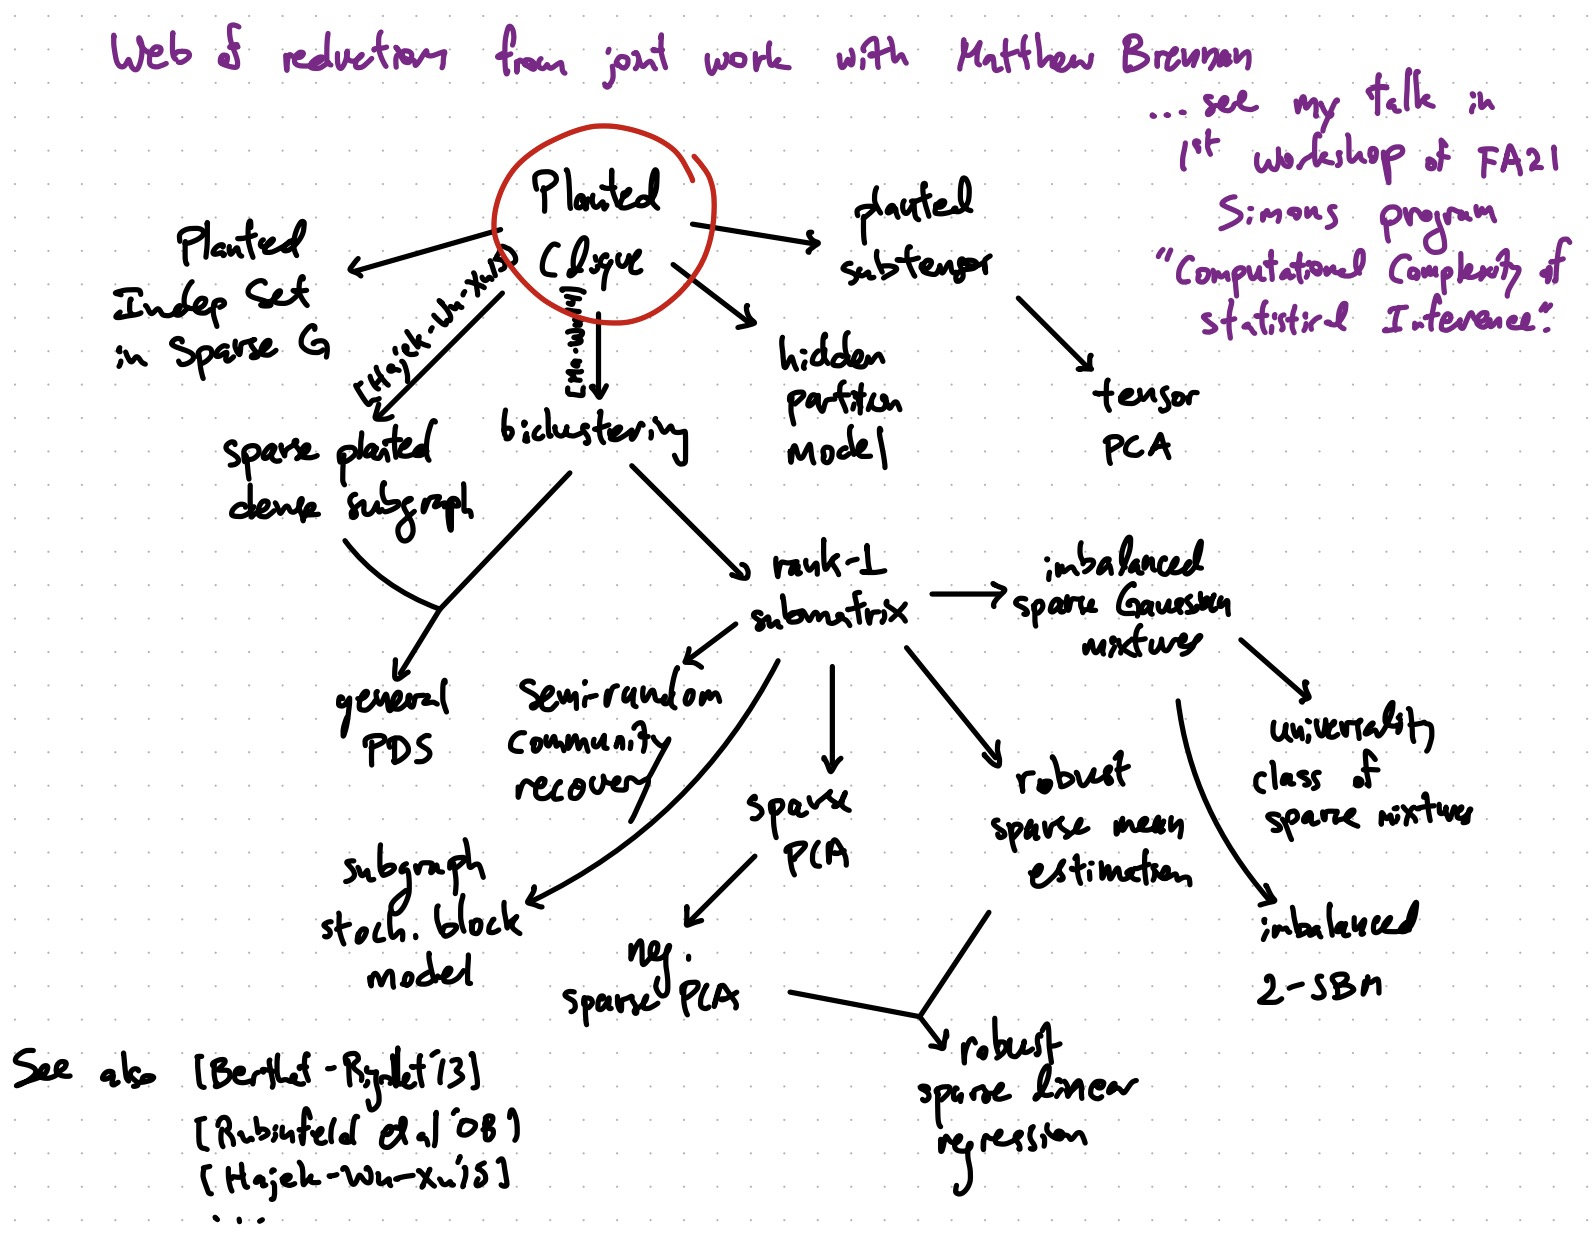
\includegraphics[width=0.55\textwidth]{web_of_redu.jpg}
    \caption{Web of reduction \xb{cite:from brysler's talk}}
    \label{web_of_redu}
\end{figure}

\begin{figure}
    \centering
    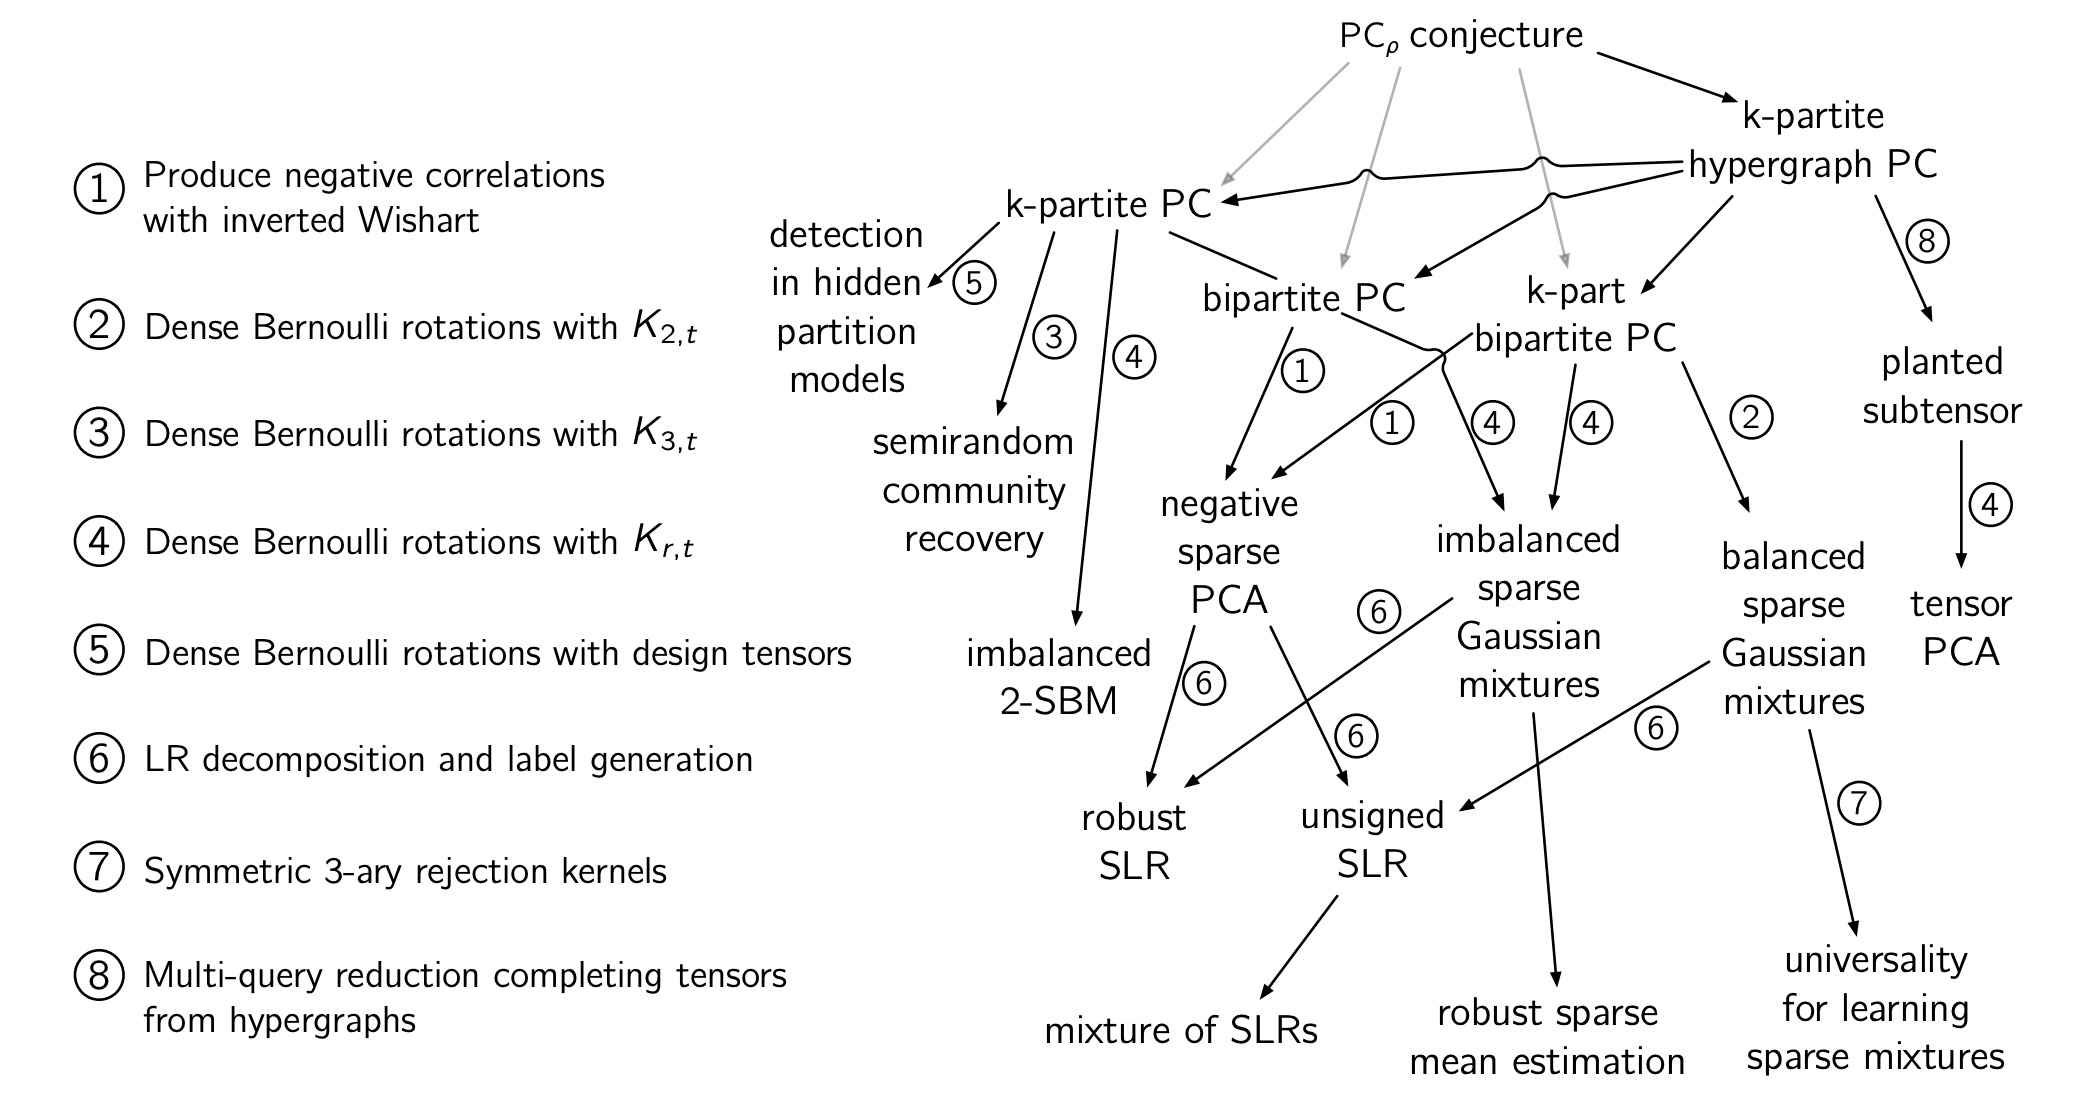
\includegraphics[width=0.7\textwidth]{web_of_redu2.jpg}
    \caption{Web of reduction  \cite{brennan2020reducibility}}
    \label{web_of_redu2}
\end{figure}


An open problem is to consider the equivalence of the problem, that is, reduction from both sides.

\textbf{Other related problems and complexities}
\begin{itemize}
    \item Communication complexity
    
    \xb{add some intro...rNLA type of papers usually emphrase model of query, but info-comp gap type of papers ususally don't? check that, e.g. what's query model of hardness conjecture of planted cliques}

    \cite{rashtchian2021averagecase} attemps to make communication problem(alice and bob) as a \textbf{new primitive}, prior to planted clique problem and its variants, under different query models. 
    
    For example, a reduction from planted clique(average-case) $PC(n,k)$ to unique disjointness(worst-case) $UD(l)$(which may be too lose since the primitive is nonrandom):
    \begin{enumerate}
        \item Given inputs $x,y\in\{0,1\}^l$ for Alice and Bob respectively.  Construct a clique partition of $K_n$ with a collection $S$ of $l$ edge-disjoint $k$-cliques, which requires $l=\Theta(n^2/k^2)$.
        \item Introduce randomness. First randomly picked the edges that aren't covered by $S$ with probability $1/2$, denote the resulting graph by $G'$. Then, each of the $k$-cliques $K_k^i$ in $S$  is randomly colored at random with 4 colors, independently of each other.
        \item Construct graph. For each $i\in[l]$, if $x_i=0$, pick all edges in $K_k^i$ with colors $1$ or $3$ as graph $G_1^i$, otherwise pick edges with colors $1$ or $2$.
        If $y_i=0$, pick all edges in $K_k^i$ with colors $1$ or $4$ as graph $G_2^i$, otherwise pick edges with colors $3$ or $4$.

        \item Let $G=G'\cup(\cup_{i\in[l]}G_1^i\oplus G_2^i)$. Then $G\sim\mc H_1$ if there is a unique $i$ such that $x_i=y_i=1$, while $G\sim\mc H_0$ if there is no such $i$. Therefore, if we can solve $PC(n,k)$ under some query model(e.g. $\mb F_2$ sketching), we need at least $\Omega(n^2/k^2)$ queries due to communication complexity.
    \end{enumerate}

    \item Randomized numerical linear algebra
    
    \xb{woodruff's paper usually map problem they care into classical problem(e.g. communication), e.g. Hutch++\cite{mmmw21}. But they don't seem to estabilish system like \cite{brennan2019reducibility}}
    
    \item Graph theory
    
    \xb{search cheng mao, jian ding's works, their problems may be reduce other problem, but first we need to abstract their math structures}

    \item 
\end{itemize}

%---------------------------------------------------
%---------------------------------------------------
\subsection{Failure of general algorithms}



%---------------------------------------------------
%---------------------------------------------------
\subsection{Phenomena in hard regime}